\documentclass[a4paper, 11pt]{report}

% Langue & Encodage
\usepackage[french]{babel} % Langue française
\usepackage[utf8]{inputenc} % Pour l'UTF-8
\usepackage[T1]{fontenc} % Césure de caractères accentués

% Police
\usepackage{lmodern} % Police standard sous LaTeX : LatinModern (alternative à la police d'origine développée par DonaldKnuth : Computer Modern)

% Mise en page
%\usepackage[top=2.5cm, bottom=2.5cm, left=2.5cm, right=2.5cm]{geometry}
\usepackage{fullpage}

% URL & Génération du PDF
\usepackage[hyphens]{url}
\usepackage[pdfauthor = {{Théo DURR, Célian HUMBERT}}, pdftitle = {{AC20 - Etudes de systèmes dynamiques non déterministes}}, pdfstartview = Fit, pdfpagelayout = SinglePage, pdfnewwindow = true, bookmarksnumbered = true,breaklinks, colorlinks, linkcolor = blue, urlcolor = black,citecolor = cyan, linktoc = all]{hyperref}

% Images
\usepackage{graphicx}
\graphicspath{ {pictures/} } % Spécifie le chemin où sont enregistrées les images

% Maths
\usepackage{amsmath}

% Création de sections personnaliséés
\newtheorem{axiome}{Axiome}

% Inclusion de PDFs
\usepackage{pdfpages}

\begin{document}
    % Première de couverture
    \begin{titlepage}
    \newcommand{\HRule}{\rule{\linewidth}{0.1mm}} % Ligne horizontale (épaisseur modifiable}
    \enlargethispage{2cm} % Réduit la taille du footer

    \begin{center}
        % En-têtes
        \textsc{\Large{}Mémoire en vue de la validation de l'unité de valeur} \\[0.5cm]
        \textsc{\large{}AC20 - Aquisition de connaissances} \\[1.5cm]

        % Titre
        \HRule \\[0.6cm]
        {\huge\bfseries{}\'Etude de systèmes dynamiques\\ non déterministes} \\[0.25cm]
        \HRule \\[1.5cm]

        % Auteurs
        \begin{flushleft}
            \Large\textbf{Auteurs :}\\[0.2cm]
                Théo \textsc{Durr} \\
                Célian \textsc{Humbert}

                \vspace{1cm} 

                \Large\textbf{Enseignant chercheur encadrant :}\\[0.2cm]
                Frédéric \textsc{Holweck}
        \end{flushleft}

        \vfill

        
\includegraphics[width=8cm]{utbm_logo.jpg} \\
        \textsc{\LARGE{}Université de Technologie de Belfort-Montbéliard} \\[1.5cm]

        \vspace{1.5cm}

        Printemps 2021

    \end{center}
\end{titlepage}

    % Avant-propos
    \chapter*{Avant-propos}
% Explication du choix du sujet, méthodologie de travail
On entend souvent parler du chaos comme l'absence d'ordre ou de logique, comme une force mystérieuse qui 
rendrait aléatoire et imprédictible certains évènements et façonnerait le monde sans que l'on puisse vraiment comprendre comment et pourquoi. Le chaos est également souvent associé avec l'effet papillon 
qui explique qu'un changement inperceptible peut avoir des conséquences de proportion complètement différentes.

Ce sont sans doute l'image populaire, le mystère et l'aspect universel du chaos qui nous ont poussé à nous intéresser à ce sujet, et à vouloir acquérir de plus amples connaissances à son propos, de plus il s'agit d'un sujet très interessant car l'étude des phénomène chaotique est un champ de recherche relativement récent qui touche à de très nombreux domaines et permet d'appréhender le monde d'une manière nouvelle et différente.  Pour se faire, nous avons utilisés diverses méthodes, évidement nous avons mené de nombreuses recherches sur le sujet afin de ce familiariser avec lui et d'avoir une meilleure idée de son ampleur et des différents domaines où l'ont peut retrouver l'intervention du chaos. 

Evidement, l'étude de la théorie du chaos dans son ensemble nous est inaccessible de part sa complexité et ses applications très nombreuses. Nous avons donc fait le choix d'étudier des phénomènes mathématiques et physiques relativement simples ou l'on peut retrouver la marque du chaos. Ses études passent bien sûr par une analyse mathématique mais également par la construction de graphiques à l'aide d'algorithmes que nous avons écrit afin de mettre en application notre compréhension et nos connaissances de ces phénomènes.



    % Remerciements
    \chapter*{Remerciements}


    % Table des matières
    % ! DISPLAY TALBEOFCONTENT
    {
    \hypersetup{linkcolor=black}
    \tableofcontents
    }

    % Introduction
    \chapter{Introduction}
Au travers de nos recherches, nous avons essayé de comprendre et d'étudier le chaos, ou appelés mathématiquement les systèmes dynamiques non déterministes. 

Bien que cet énoncé puisse paraître compliqué, il désigne simplement tout système dynamique dont on ne peut pas déterminer précisément l'évolution sans une connaissance parfaite de ses conditions initiales, il s'agit de la principale caractéristique des systèmes chaotiques. Nous avons notamment étudié deux célèbres systèmes exhibant ces caractéristiques : La fonction logistique, ainsi que les célèbres équations de Lorenz qui sont l'un des \og point de départ \fg{} de la théorie du chaos et à qui sont également à l'origine de l'expression "effet papillon".

L'origine de ce nom vient d'une de ses conférences concernant ses travaux, et qui avait pour titre "Does the flap of a butterfly’s wings in Brazil set off a tornado in Texas ?" (Traduit par \og Le battement d'ailes d'un papillon au Brésil peut-il déclencher une tornade au Texas ?\fg{}). Nous essayerons d’apporter des éléments de réponse à cette célèbre question. Les deux systèmes mentionnés précédemment présentent une forte dépendance aux conditions initiales, mais ils possèdent une autre caractéristique que l'on retrouve souvent dans les systèmes chaotiques: ils possèdent une dimension fractale. Vous trouverez donc tout au long de ce document l'analyse et l'explication du comportement de ses systèmes afin de mieux comprendre ce qu'est "scientifiquement" le chaos.
  


    % Partie fonction logistique
    \chapter{Fonction logisitque}
% Faire un historique
Cette fonction a été introduite par Pierre François Verhlust (1804-1849). Il s'agit d'un modèle de croissance des populations proposé en réponse au modèle de Malthus, qui proposait un taux d'accroissement constant, sans frein conduisant à une croissance exponentielle de la population.

Si on note $t\mapsto x(t)$, la fonction qui représente la population au temps $t$. Le modèle de Malthus se traduit mathématiquement de la manière suivante : $x'(t)=x(t)$. Les solutions d'un tel modèle sont des \textbf{exponentielles}.

On peut voir ici que le modèle de Verhlust est plus fin : il prend en compte l'effet de \og surpopulation\fg{} qui conduit à une raréfication des ressources et donc à la diminution de la population. Mathématiquement, cela conduit à étudier la fonction $x'=\lambda x(1-x)$ : le taux d'accroissement diminue quand $x$ augmente à cause du facteur $(1-x)$.

\begin{axiome}[La fonction logisitque (Verhlust)]
Soit $\lambda \in [0;4]$, on considère la fonction logistique
\[
    f_\lambda : \left|
    \begin{array}{ccc}
        [0;1] &\longrightarrow& [0;1] \\
        x &\mapsto& \lambda x(1-x)
    \end{array}
    \right.  
\]
\end{axiome}

Nous allons dans notre cas, étudier une version discrète de ce modèle, c'est-à-dire à l'aide de suites. Nous allons donc étudier l'évolution des suites récurrentes définies par :
\[
    \left\{
    \begin{array}{rcl}
            u_0 &\in& [0;1] \\
            u_{n+1} &=& f_\lambda(u_n)
    \end{array}
    \right.
\]

\section{Analyse graphique \& expérimentation numérique}
\subsection{Etude générale}


\subsection{Etude de la version discrète}
On cherche à observer numériquement le comportement de la suite $(u_n)$. Pour cela, nous avons observé le comportement des $30$ premiers termes de la suite, pour $u_0 = 0.5$ et $\lambda\in\{0,5; 1,5; 2,5; 3,2; 3,5\}$.

\begin{figure}[!ht]
    \begin{center}
        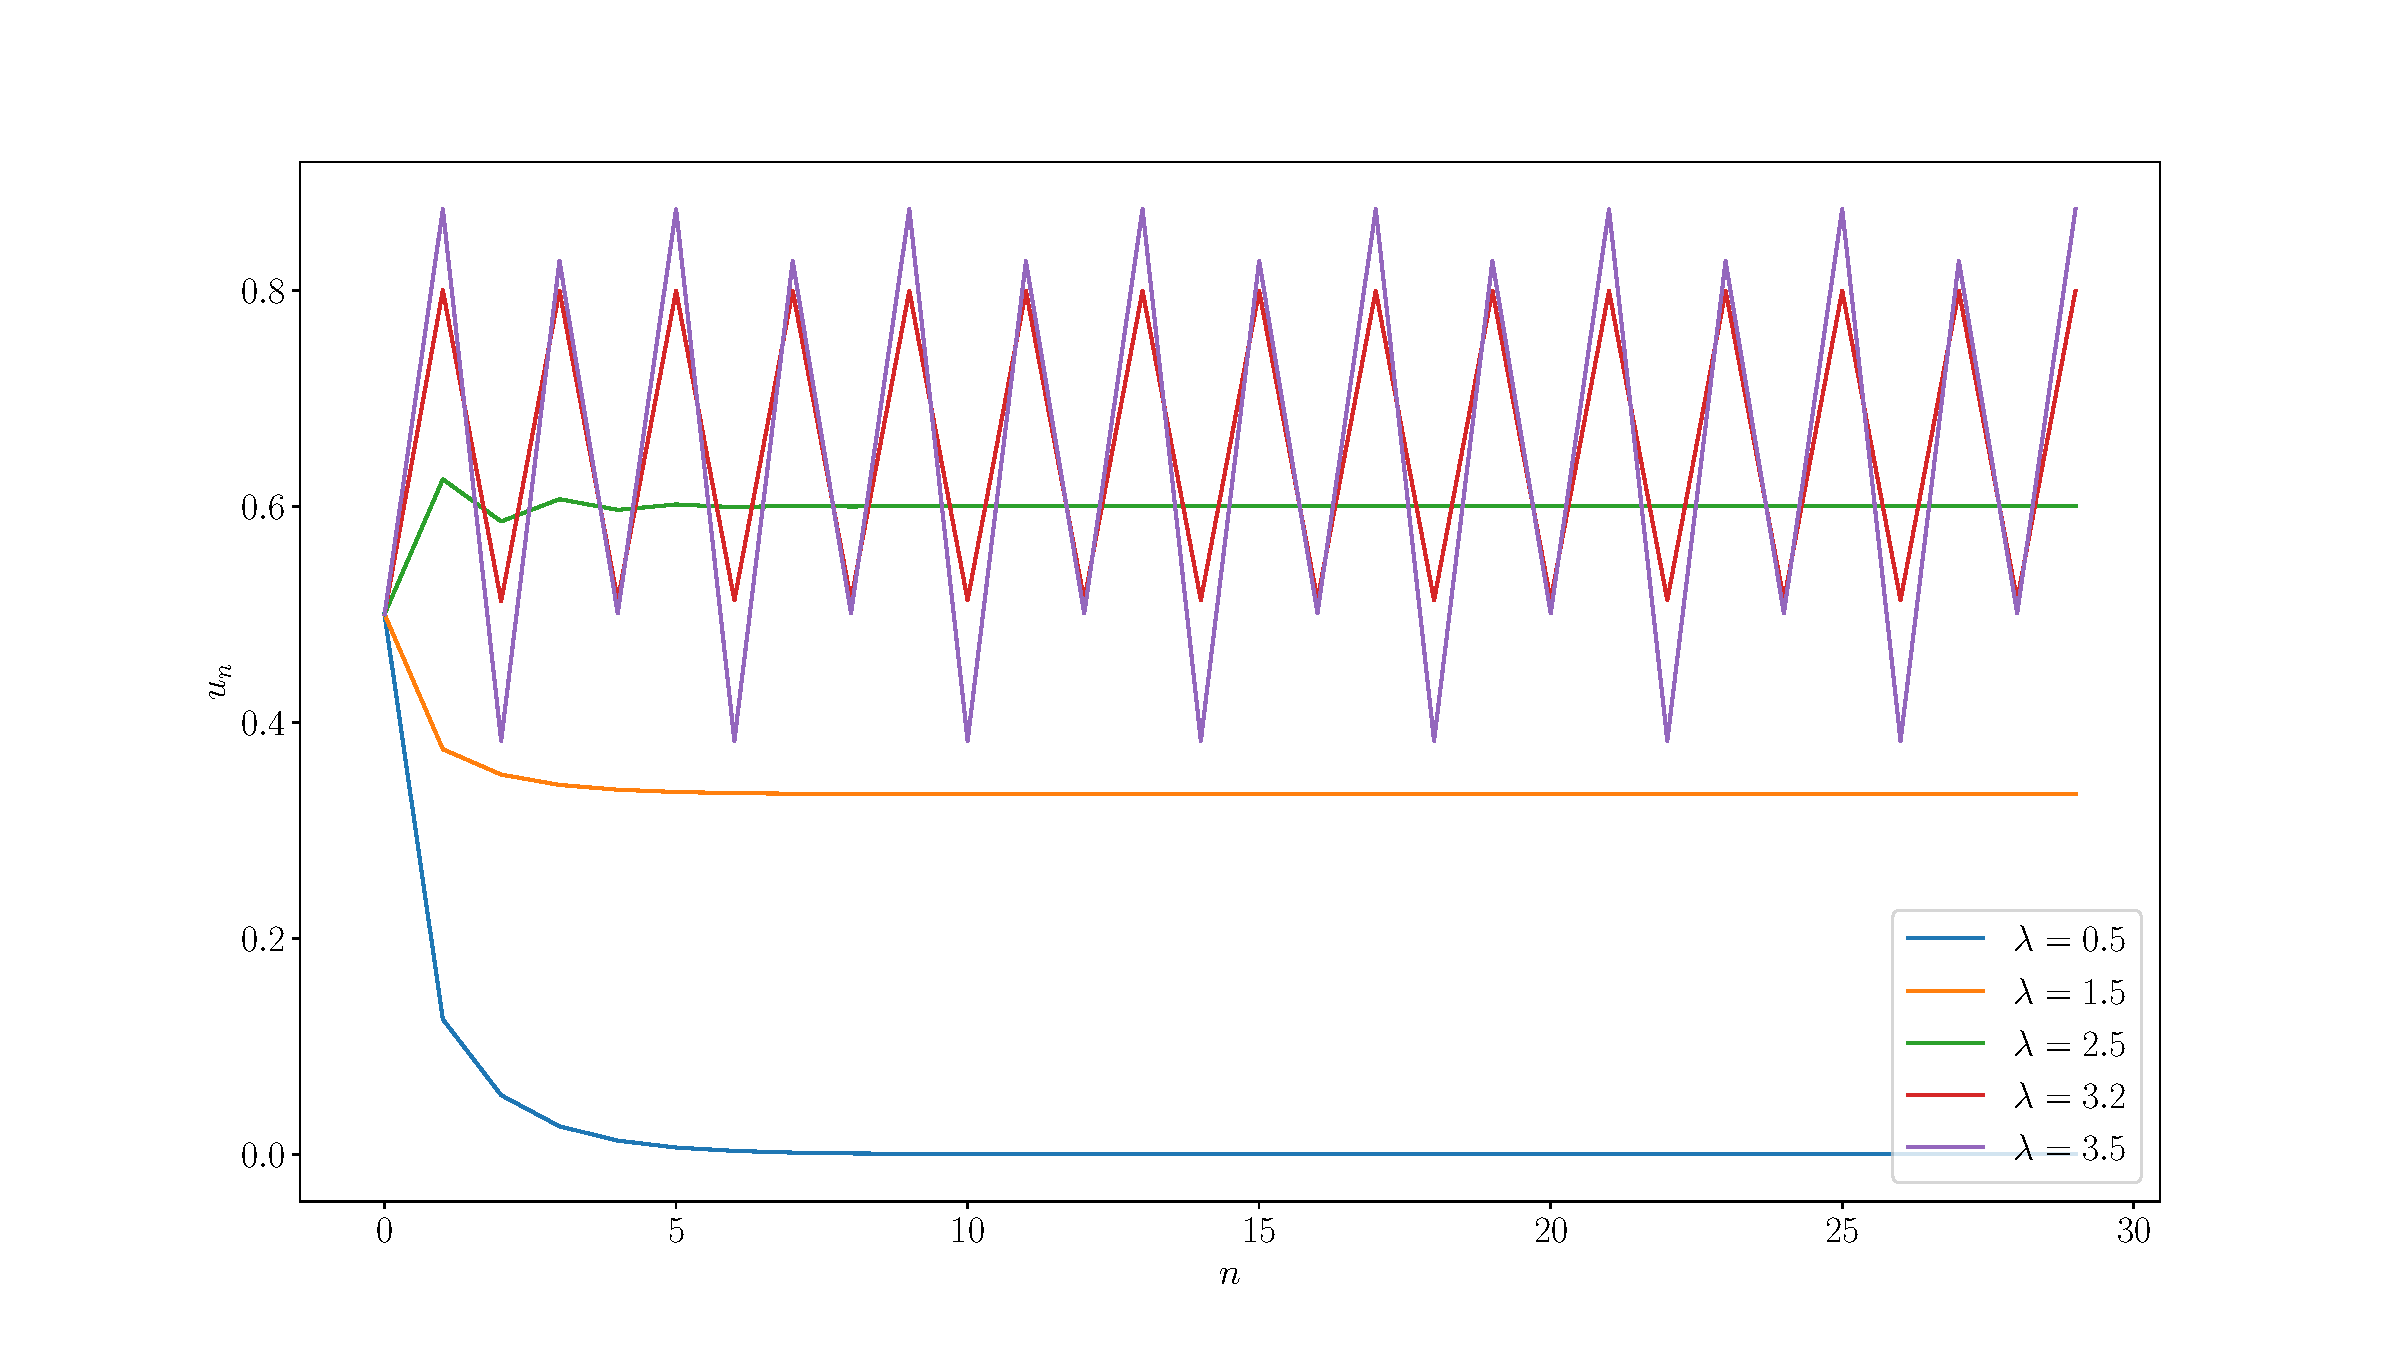
\includegraphics[width=\textwidth]{experimentation_numerique.pdf}
    \end{center}
    \caption{Etude de la suite logistique pour différentes valeurs de $\lambda$}
    \label{fig:etude_lambdas}
\end{figure}
On peut voir sur la figure \ref{fig:etude_lambdas} que pour les valeurs de $\lambda\in\{0,5; 1,5; 2,5\}$, la suite $(u_n)$ est convergente, et converge respectivement vers (environ) $0; 0,33$ et $0,6$. On peut déceler un comportement particulier pour les valeurs de $\lambda \in\{3,2; 3,5\}$ : elles semblent converger périodiquement vers deux points. On peut trouver les suites extraites afin de donner une valeur approchée de leurs limites.

Pour $\lambda = 3,2$, la suite des termes pairs $(u_{2n})$ converge vers approximativement $0,51$. Tandis que la suite des termes impairs $(u_{2n+1})$ converge vers approximativement 0,80. De même pour $\lambda = 3,5$ où, les limites des suites extraites sont (approximativement) $0,4$ et $0,9$.

\subsection{Sensibilité aux conditions initiales}
Pour cette partie, fixons $\lambda = 4$ et étudions la suite logistique avec $u_0 = 0,4$ et $u'_0 = 0,4 + 10^{-8}$. On remarque sur la figure \ref{fig:etude_u0} (page \pageref{fig:etude_u0}) que les courbes se superposent parfaitement jusqu'au 17\ieme{} terme. Au delà, les courbes commencent à se dissocier et se dissocient rapidement.

\begin{figure}[!ht]
    \begin{center}
        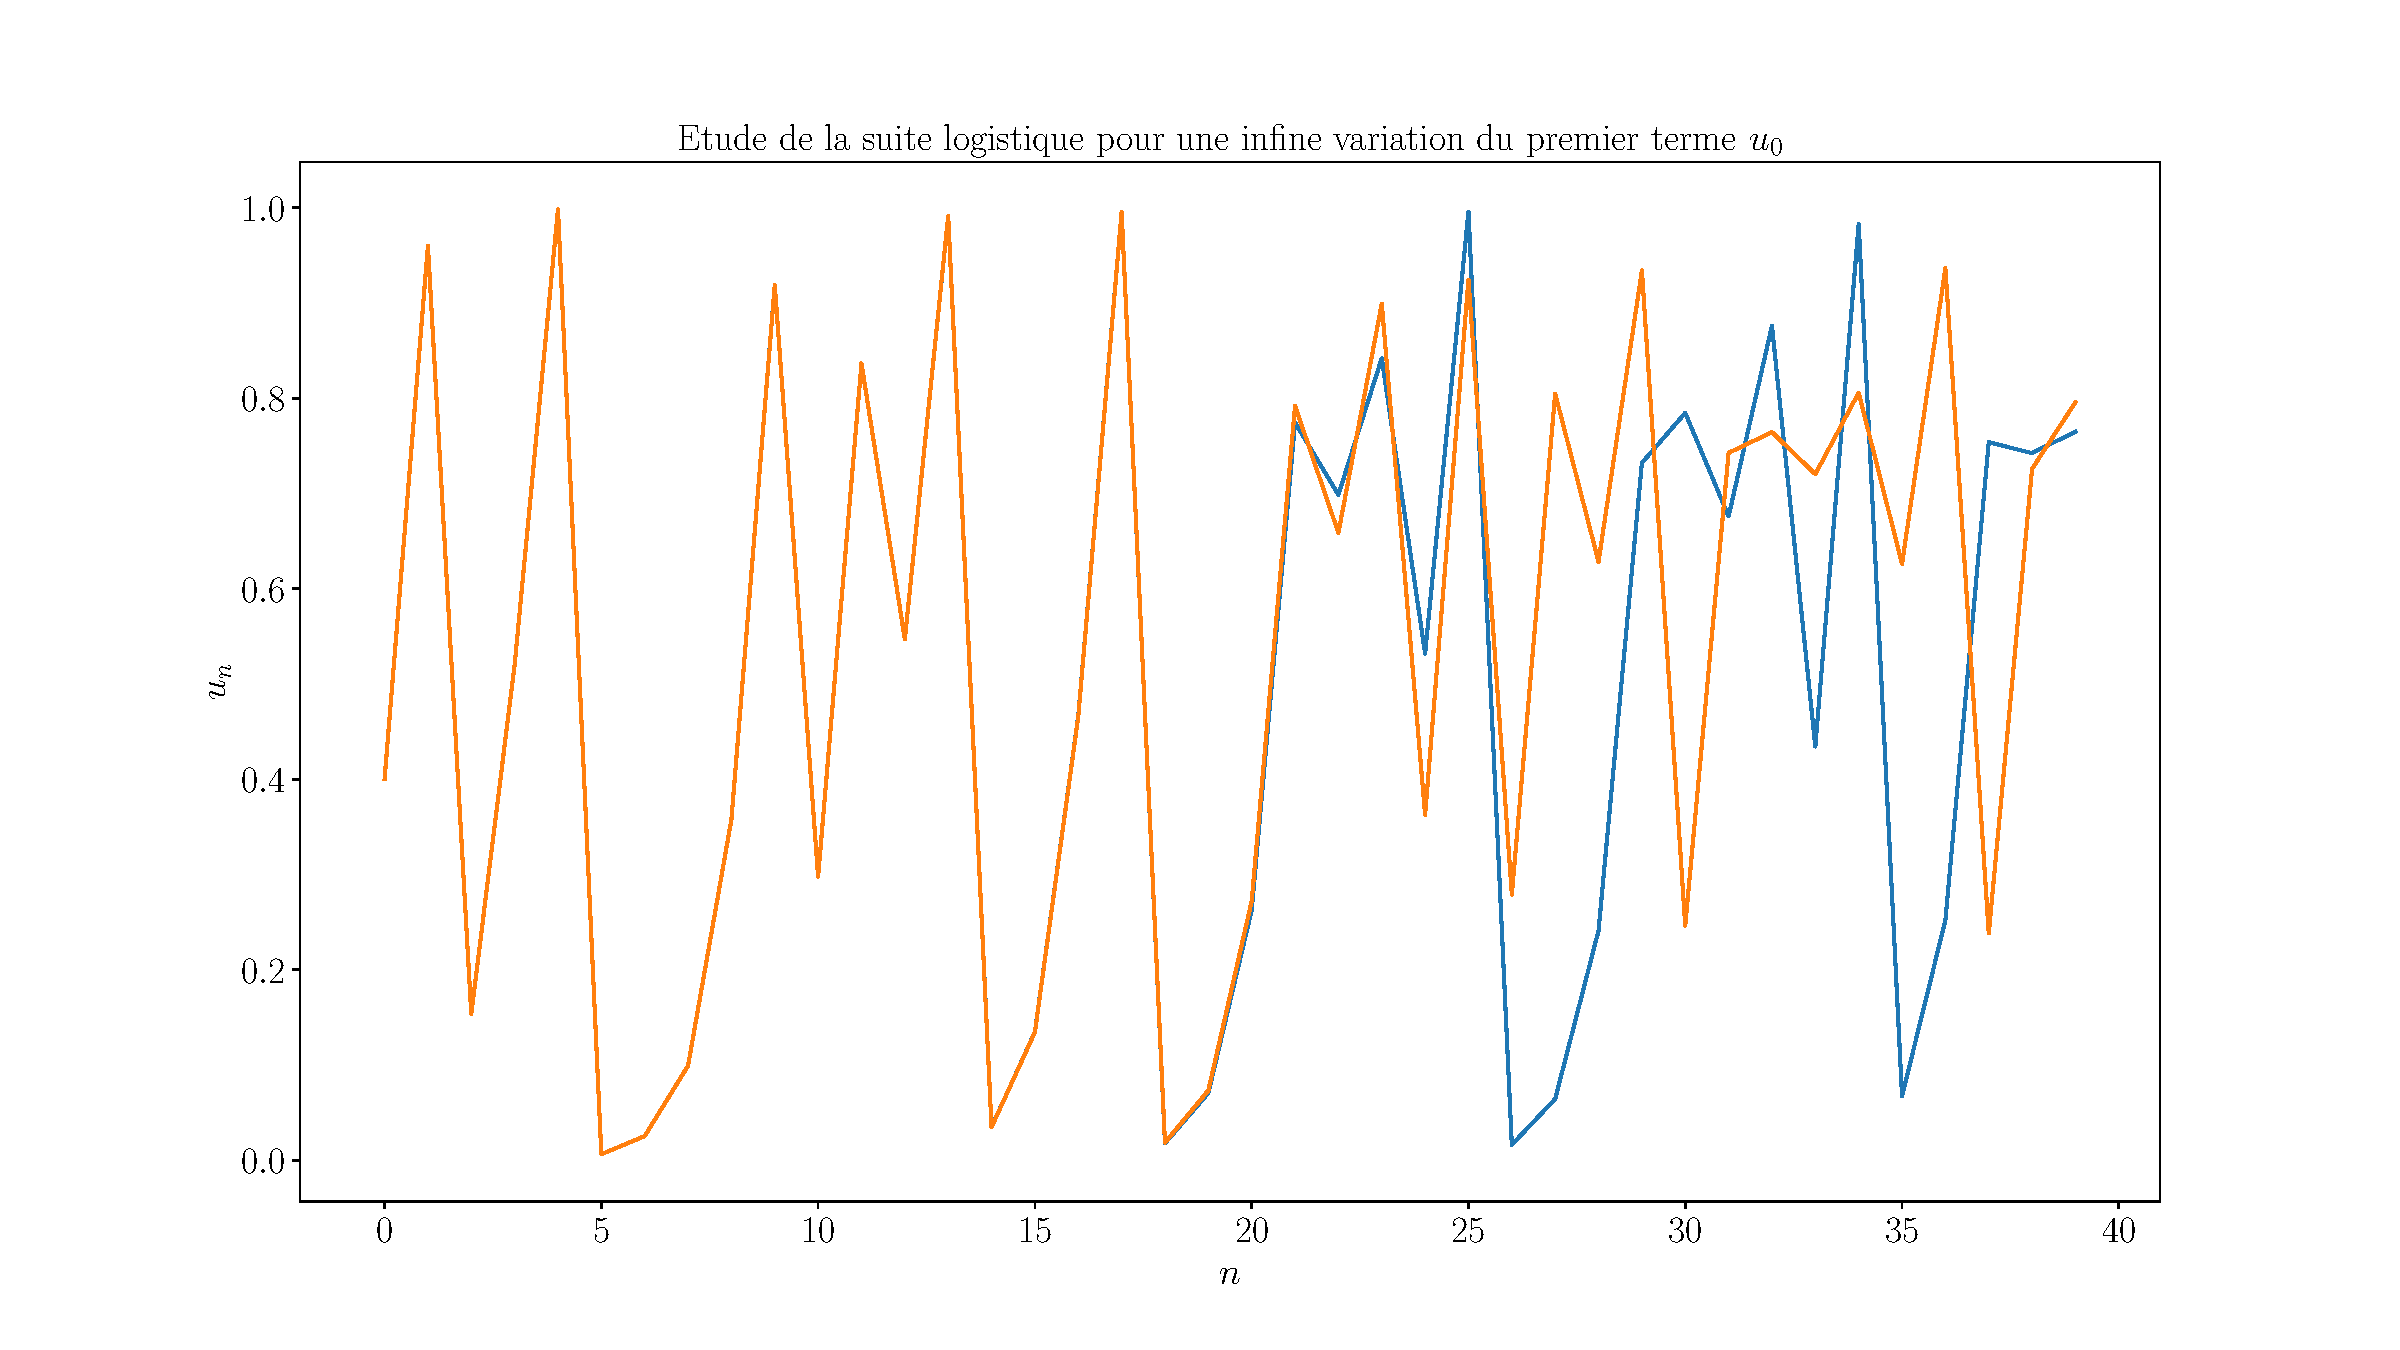
\includegraphics[width=\textwidth]{variation_u0.pdf}
    \end{center}
    \caption{Etude de la suite logistique pour une infime variation du premier terme $u_0$}
    \label{fig:etude_u0}
\end{figure}

Cette partie illustre le fait que pour $\lambda = 4$, la suite $(u_n)$ a une forte sensibilité aux conditions initiales. Une infine variation des conditions initiales (ici $0,00000001$) a des conséquences énormes sur les résultats : le système est donc \textbf{chaotique}, et introduit la notion d'\textit{effet papillon}.

% Transition

\section{\'Etude mathématique}
\subsection{\'Etude du cas : \texorpdfstring{$\lambda \leq 1$}{Lg}}
Durant toute cette partie, on supposera $\lambda \leq 1$.

En plus des études graphiques, nous allons maintenant nous intéresser à des preuves mathématiques validant les hypothèses que nous aurions pu émettre.
Tout d'abord, nous aurons besoin des bornes de $f_\lambda$ durant toute la suite de l'étude. Montrons donc que $f_\lambda([0;1])\in[0;1]$ :

Etudions la fonction $f_\lambda(x)$ :
\[
    f_\lambda(x)=\lambda x(1-x) = \lambda x - \lambda x^2
\]

Calculons son discriminant $\Delta$ :
\[
    \begin{array}{rcl}
        \Delta &=& \lambda^2-4\times\lambda\times 0 \\
        &=& \boxed{\lambda^2 > 0}
    \end{array}
\]
Il existe donc deux racines $x_1$ et $x_2$ :
\[
    \begin{array}{rcl}
        x_1 &=& \dfrac{- \lambda-\sqrt{\lambda^2}}{-2\lambda} = \dfrac{-2\lambda}{-2\lambda} = \boxed{1} \\
        x_2 &=& \dfrac{- \lambda+\sqrt{\lambda^2}}{-2\lambda} = \boxed{0}
    \end{array}
\]
On voit donc que $f_\lambda$ est \textbf{positive} sur l'intervalle $[0;1]$. Calculons les coordonnées du sommet afin de s'assurer que son ordonnée ne soit pas supérieure à $1$ :
\begin{axiome}[Coordonnées du sommet d'une parabole]
    Soit $f(x) = ax^2+bx+c$ un polynôme du second degré. Les coordonnées du sommet $S$ de la courbe représentative de $f$ sont
    \[
          S\left(-\frac{b}{2a};f\left(-\frac{b}{2a}\right)\right)
    \]
\end{axiome}

Notons, $S_\lambda$ le sommet de la courbe représentative de $f_\lambda$. L'ordonnée de $S_\lambda$ vaut :
\[
    f\left(\dfrac{1}{2}\right) = \dfrac{\lambda}{4}
\]

Calculons les bornes de $y$ en fonction de $\lambda$ :
\[
    \begin{array}{rcccl}
        0 &\leq& \lambda &\leq& 1 \\
        \Longleftrightarrow 0 &\leq& \dfrac{\lambda}{4} &\leq& \dfrac{1}{4}
    \end{array}
\]

Comme $\frac{1}{4} < 1$, le sommet ne dépassera jamais $1$. Donc $\boxed{f([0;1]) \subset[0;1]}$. Cela ne pose pas non plus de soucis lorsqu'on étudie la version discrète à l'aide de suites, car comme $u_0 \in[0;1]$ et que $f_\lambda([0;1])\subset[0;1]$, alors $f_\lambda(u_n) = u_{n+1}\in[0;1]$.


Nous voyons graphiquement que pour $\lambda \leq 1$, la suite semble converger vers $0$. Prouvons cela mathématiquement en étudiant la monotonie de la suite $(u_n)$.
$$
    \begin{array}{rcl}
        u_{n+1}-u_n &=& \lambda u_n(1-u_n)-u_n \\
                    &=& u_n(\lambda(1-u_n)-1) \\
    \end{array}
$$
Or,
$$
    \begin{array}{rcl}
        &&u_n \leq 1 \\
        &\Longleftrightarrow& 1 - u_n \leq 1 \\
        &\Longleftrightarrow& \lambda(1 - u_n) \leq 1 \\
        &\Longleftrightarrow& \lambda(1 - u_n) - 1 \leq 0 \\
        &\Longleftrightarrow& u_n(\lambda(1 - u_n) - 1) \leq 0 \\
    \end{array}
$$
La suite est donc \textbf{décroissante}. De plus, elle est minorée par $0$. Elle est donc bien \textbf{convergente}. Il serait également intéressant de connaître la limite de la suite $(u_n)$, élément crucial afin de déterminer son comportement en fonction de $\lambda$.
\begin{axiome}[Point fixe]
    En mathématique, pour une application $f$ d'un ensemble $E$ dans lui-même, un élément $x$ de $E$ est un \textbf{point fixe de $f$} si
    \[
        f(x) = x  
    \]
    Graphiquement, les points fixes d'une fonction $f$ (d'une variable réelle, à valeurs réelles) s'obtiennent en traçant la droite d'équation $y = x$ : tous les points d'intersection de la courbe représentative de $f$ avec cette droite sont alors les points fixes de $f$.
\end{axiome}
\begin{axiome}[Point fixe et convergence]
    On considère une fonction continue $f : E \longrightarrow E$ et $(u_n)$ une suite récurrente définie par sa valeur initiale $u_0$ et par la relation de récurrence $u_{n+1} = f(u_n)$.
    
    Si $(u_n)$ converge vers un élément $l$ de $E$, la limite $l$ est nécessairement un point fixe de $f$.
\end{axiome}

Afin de trouver la limite de la suite $(u_n)$, nous allons donc calculer les points fixes de $f_\lambda$ pour $\lambda \leq 1$. C'est à dire, résoudre l'équation $f_\lambda(x) = x$:
\[
    \begin{array}{rcl}
        && f_\lambda(x) = x \\
        &\Longleftrightarrow& \lambda x(1-x)-x = 0 \\
        &\Longleftrightarrow& x(\lambda(1-x)-1) = 0 \\
        &\Longleftrightarrow& -\lambda x(-(1-x)+\frac{1}{\lambda}) = 0 \\
        &\Longleftrightarrow& -\lambda x(x-1+\frac{1}{\lambda}) = 0 \\
        &\Longleftrightarrow& -\lambda x(x-(1-\frac{1}{\lambda})) = 0 \\
    \end{array}
\]

Par déduction directe, on peut trouver les solutions de l'équation
$$
    f_\lambda(x) = x \Longleftrightarrow \left\{
            \begin{array}{rcl}
                    x &=& 0 \\
                    x &=& 1 - \dfrac{1}{\lambda}
            \end{array}
        \right.
$$
Cette équation a donc deux solutions : $x_1 = 0$ et $x_2 = 1 - \frac{1}{\lambda}$. Or, $\lambda \leq 1$, donc $x_2 \leq 0$. $x_2$ n'est donc pas un élément de $E$, il ne s'agit donc pas d'un point fixe. Ainsi, pour $\lambda \leq 1$, la fonction $f_\lambda$ possède un unique point fixe sur $[0,1]$ qui est $x = 0$. Nous avons montré précédemment que la suite $(u_n)$ tend vers une limite $l$. Par construction de $(u_n)$ et par continuité de $f_\lambda$, on a 
$$
    \left\{
        \begin{array}{rcl}
                u_{n+1} &=& f(u_n) \\
                u_{n+1} &\longrightarrow& l \\
                f(u_n)  &\longrightarrow& f(l) \\
        \end{array}
    \right.
$$
On en déduit donc que $\boxed{l = f(l)}$, c'est-à-dire que $l$ est un \textbf{point fixe} de $f_\lambda$, et $l=0$.

\subsection{\'Etude du régime stationnaire : \texorpdfstring{$1 < \lambda < 3$}{Lg}}
\subsection{\'Etude d'un cycle d'ordre 2 : \texorpdfstring{$3 < \lambda < 1+\sqrt{6}$}{Lg}}

\section{Le diagramme de bifurcation}

    % Partie lorenz
    \chapter{Les attracteurs de Lorenz}
Tout d’abord commençons par définir rapidement et sans rentré dans les détails mathématiques ce qu’est un attracteur,
 il s’agit d’un ensemble ou d’un espace vers lequel un système dynamique évolue de manière
 irréversible en l’absence de perturbation, le concept d’attracteur est l’une des bases de la théorie du chaos. 
 Dans cette partie nous allons nous concentrer sur l’attracteur de Lorenz, il s’agit d’un attracteur
représentant l’évolution du système dynamique différentiel de Lorenz.

Le système de Lorenz s'écrit: 
\[
    \left\{
    \begin{array}{rcl}
        \dfrac{dx}{dt}&=&\sigma[y(t)-x(t)]\\
        \dfrac{dy}{dt}&=&\rho x(t)-y(t)z(t)\\
        \dfrac{dz}{dt}&=&x(t)y(t)-\beta z(t)\\
    \end{array}
    \right.
\]
Ces équations sont un modèle très simplifier crée par Lorenz pour modélisé le fonctionnement 
de l’atmosphère terrestre. Il a décidé de cherché un modèle simple car 
les équations décrivant l’atmosphère de façon précise était beaucoup trop compliqué à résoudre
 numériquement à l’époque de Lorenz et il souhaitais pouvoir étudié  le phénomène de convection
de Rayleigh-Bénard à l’aide de son modèle simplifié.

Dans ces équations: \\
$\sigma$  correspond au nombre de Prandtl, il s'agit d'un nombre sans dimension obtenu en calculant le rapport entre la diffusivité de la quantité de mouvement et ça diffusivité thermique.\\\\
$\rho$    correspond au nombre de Rayleigh, il s'agit d'une valeur utilisé en mécanique des fluides, il permet de caractérisé le transfert de chaleur au sein d'un fluide \\\\
$\beta $  est une valeur dépendand de la couche de l'atmosphère\\\\
$x(t)$    

\section{Dimension mathématique}

\section{Dimension expérimentale}

    % Partie fractales
    \chapter{Les fractales}
\label{chapter:fractales}
Les fractales sont très liée au chaos, ont retrouve souvent des formes fractales dans les système au comportement chaotique, mais avant de faire le lien avec les parties précédente définission rapidement ce qu'est une fractale: En mathématique une fractale est un objet qui présente une structure similaire indépendament de sont échelle, autrement dit une structure sur laquelle ont peut zoomer indéfiniment et retrouvé la structure de départ.

\section{Fractale d'un diagramme de bifurcation}

\section{Fratacle de l'attracteur de Lorenz}
Le cas de l'attracteur de Lorenz est particulié en ce qui concerne les fractales car ça dimension fractale n'est pas directement observable sur ça représentation graphique, la première preuve de sa dimension fractale à été faite purement mathématiquement par... et ça première observation a été possible en... en traçant l'attracteur et en concervant 100 chiffre apès la virgule.

    % Conclusion
    \chapter{Conclusion}

    % Annexes
    \begin{appendices}
    \renewcommand\thefigure{\thesection.\arabic{figure}}
    \appendixheaderon
    \section{Graphiques}
    \label{ann:graphiques}

    \subsection{Fonction logistique}
    \begin{figure}[ht]
        \centering
        \label{ann:cycles}
        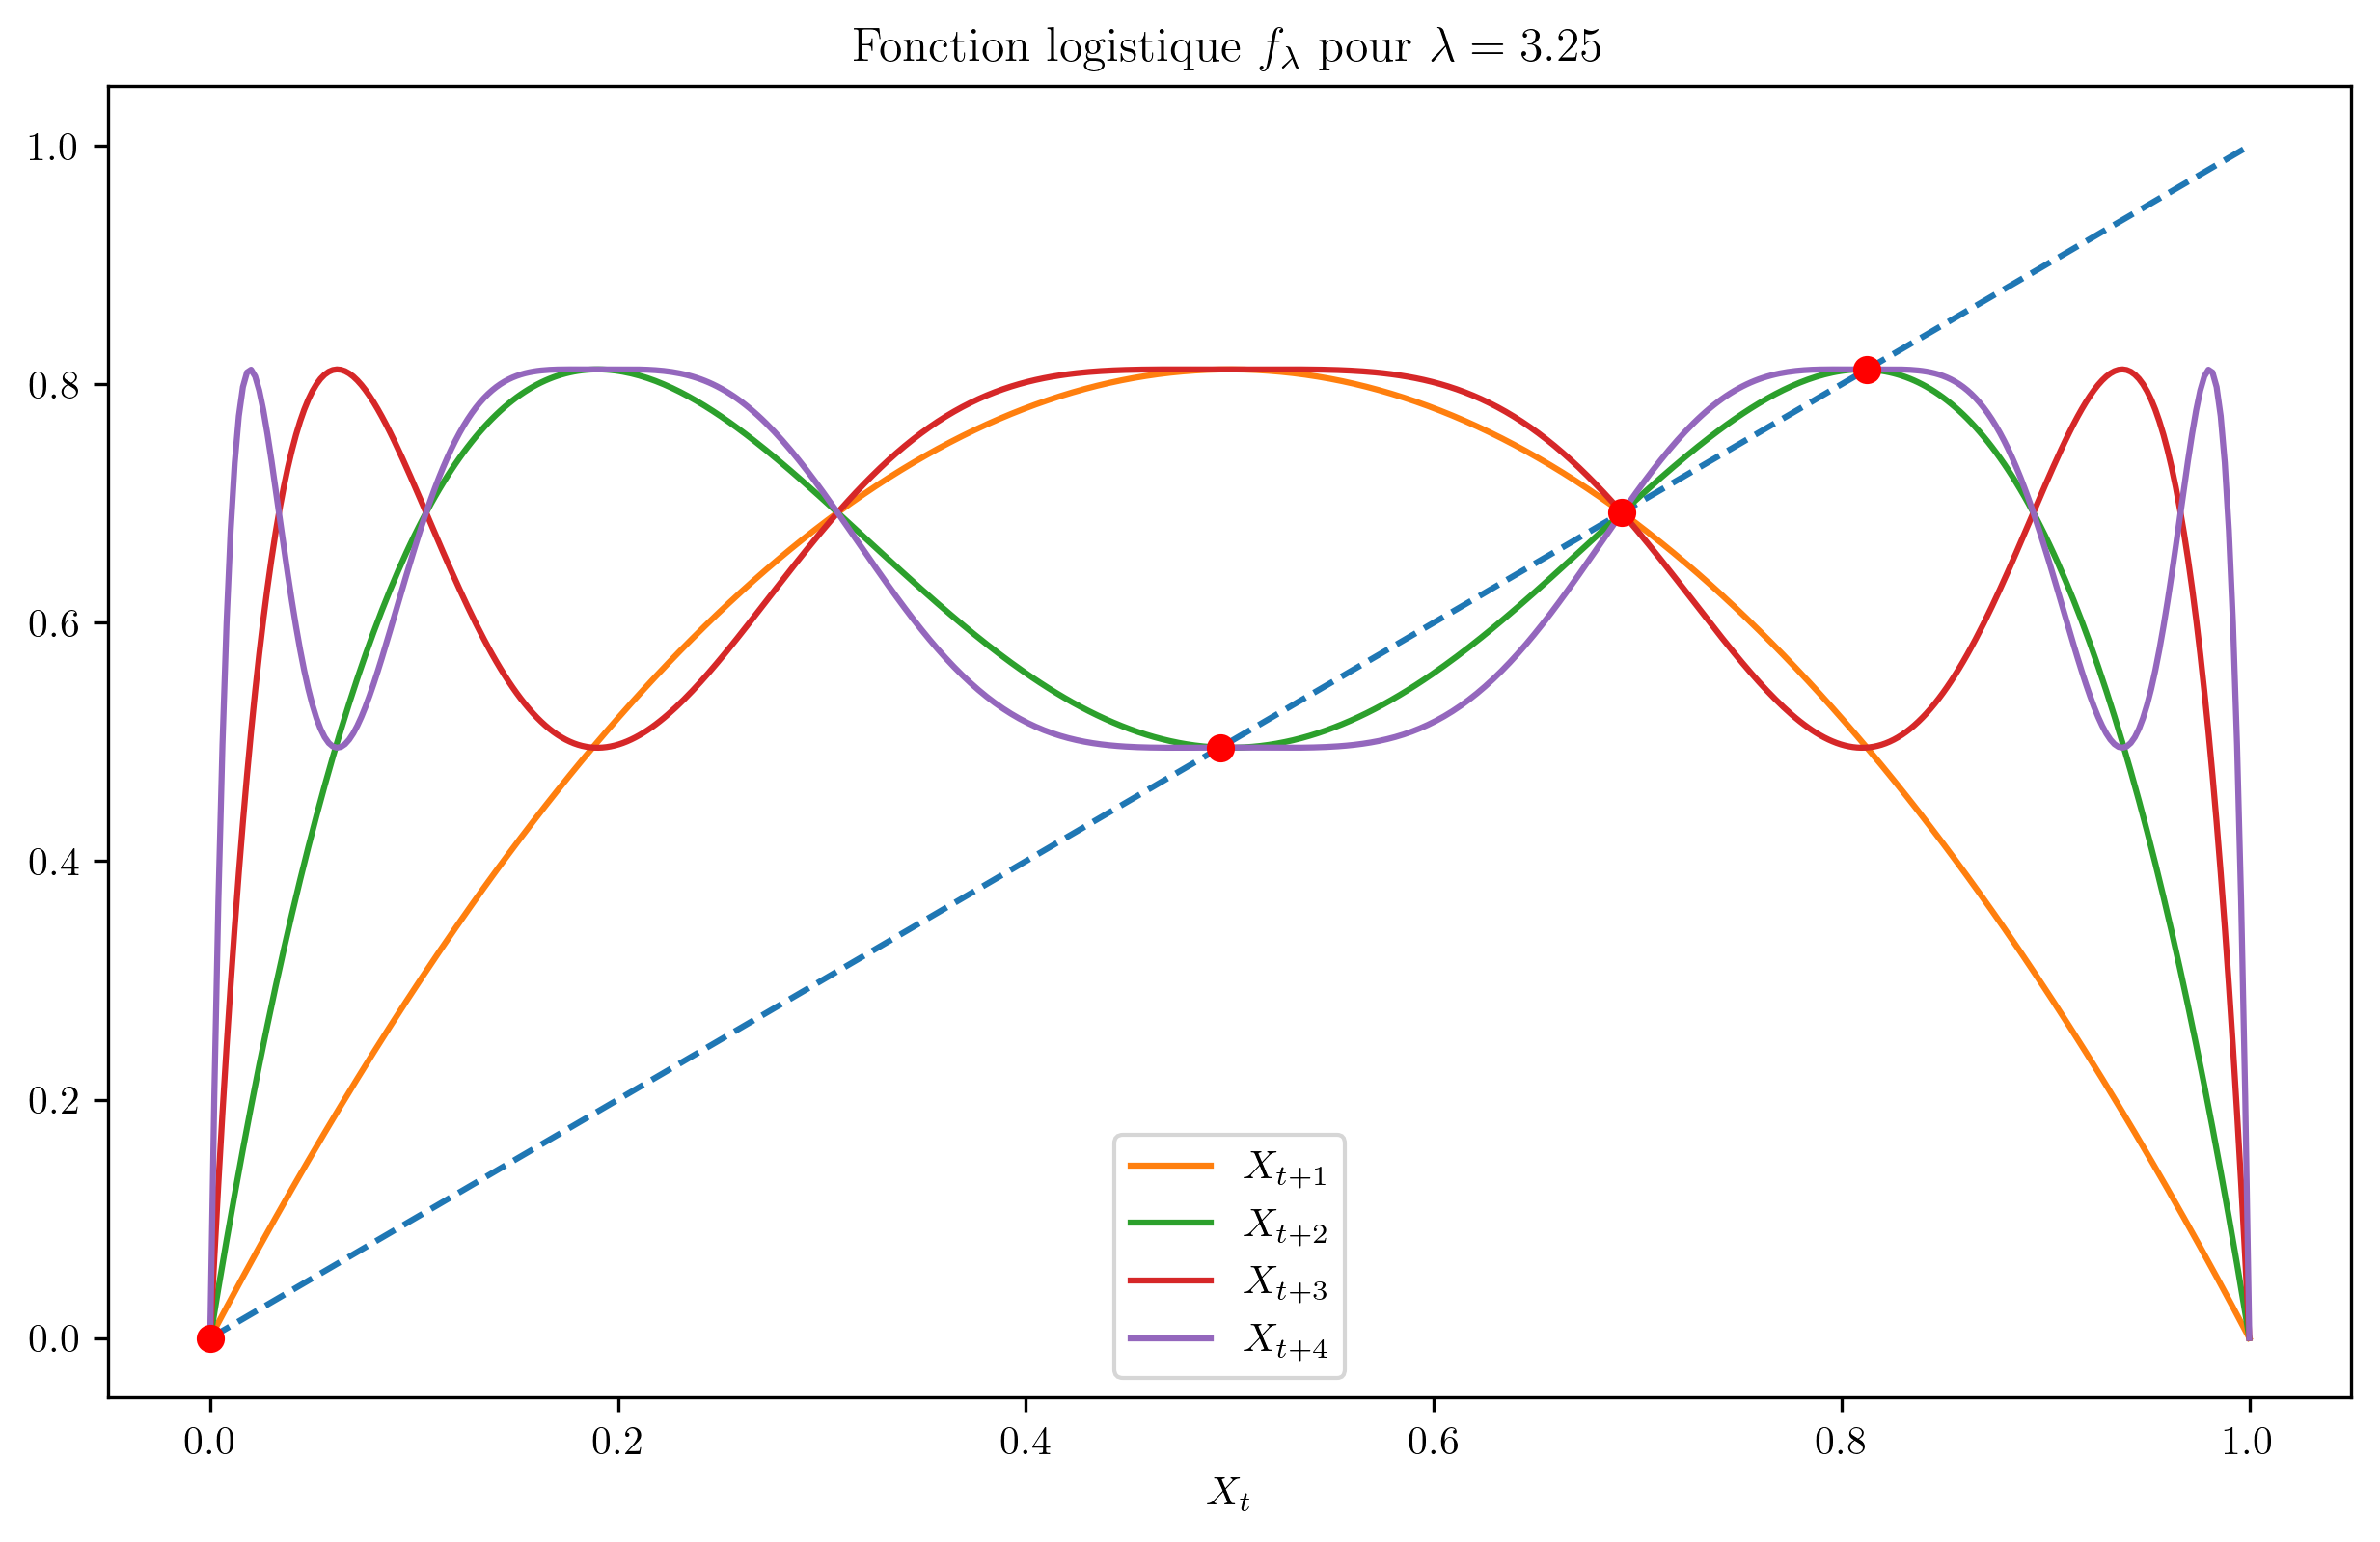
\includegraphics[width=\textwidth]{fct_log_recap.png}
        \caption{Fonction Logistique}
    \end{figure}

    \newpage
    \section{Codes python}
    \label{ann:code}

    \subsection{Génération de la fonction logistique}
    \begin{minted}{python}
# Taux d'accroissement (lambda)
a = 3.25
# Génération du vecteur des abscisses
x = np.linspace(0,1,500)
# Génération du vecteur des ordonnées
delta = x
y1 = logistical(x, a)
y2 = logistical(y1, a)
y3 = logistical(y2, a)
y4 = logistical(y3, a)

# Création de la figure (taille en pouces optionnelle)
fig = plt.figure(figsize=(10,6), dpi=300)

ax = fig.add_subplot(1,1,1)

# Génération des courbes
ax.plot(x, delta, '--')
ax.plot(x, y1, label = '$X_{t+1}$')
ax.plot(x, y2, label = '$X_{t+2}$')
ax.plot(x, y3, label = '$X_{t+3}$')
ax.plot(x, y4, label = '$X_{t+4}$')

# Génération des points fixes
stable_points = [0, 1-(1/a)]
if(a > 3):
    stable_points.append((a+1-np.sqrt((a+1)*(a-3)))/(2*a))
    stable_points.append((a+1+np.sqrt((a+1)*(a-3)))/(2*a))

for point in stable_points:
    plt.plot(point, point, 'ro')

# Configuration du graphique
ax.set_xlabel('$X_t$')
ax.set_title('Fonction logistique $f_\lambda$ pour $\lambda = {0}$'.format(a))
ax.legend(loc="lower center")

plt.show()
    \end{minted}
    \newpage
    \subsection{Génération des graphiques en toile d'arraignée}
    \begin{minted}{python}
# Figure dpi
dpi = 72

def plot_cobweb(f, r, x0, nmax=40):
    """Make a cobweb plot.

    Plot y = f(x; r) and y = x for 0 <= x <= 1, and illustrate the behaviour of
    iterating x = f(x) starting at x = x0. r is a parameter to the function.

    """
    x = np.linspace(0, 1, 500)
    fig = plt.figure(figsize=(600/dpi, 450/dpi), dpi=dpi)
    ax = fig.add_subplot(111)

    # Plot y = f(x) and y = x
    ax.plot(x, f(x, r), c='#444444', lw=2)
    ax.plot(x, x, c='#444444', lw=2)

    # Iterate x = f(x) for nmax steps, starting at (x0, 0).
    px, py = np.empty((2,nmax+1,2))
    px[0], py[0] = x0, 0
    for n in range(1, nmax, 2):
        px[n] = px[n-1]
        py[n] = f(px[n-1], r)
        px[n+1] = py[n]
        py[n+1] = py[n]

    # Plot the path traced out by the iteration.
    ax.plot(px, py, c='b', alpha=0.7)

    # Annotate and tidy the plot.
    ax.minorticks_on()
    ax.grid(which='minor', alpha=0.5)
    ax.grid(which='major', alpha=0.5)
    ax.set_aspect('equal')
    ax.set_xlabel('$x$')
    ax.set_ylabel(f.latex_label)
    ax.set_title('$x_0 = {:.1}, \lambda = {:.2}$'.format(x0, r))

    #plt.savefig('cobweb_{:.1}_{:.2}.png'.format(x0, r), dpi=dpi)
    plt.show()

class AnnotatedFunction:
    """A small class representing a mathematical function.

    This class is callable so it acts like a Python function, but it also
    defines a string giving its latex representation.

    """
    def __init__(self, func, latex_label):
        self.func = func
        self.latex_label = latex_label

    def __call__(self, *args, **kwargs):
        return self.func(*args, **kwargs)

# The logistic map, f(x) = rx(1-x).
func = AnnotatedFunction(lambda x,r: r*x*(1-x), r'$\lambda x(1-x)$')

plot_cobweb(func, 2.5, 0.5)
    \end{minted}
    \newpage
\subsection{Génération du diagramme de bifurcation}
\begin{minted}{python}
FIGSIZE = (16,9)
DPI = 240   # 240 For 4K, 80 for 720p

BORNE_INF = 0
BORNE_SUP = 4

def simulogi(x0,N,R):
    f = lambda x: R*x*(1-x)
    x = np.zeros(N)
    x[0] = x0
    for i in range(1,N):
        x[i]=f(x[i-1])
    return x


N = 30000
Imin = 100  # plot starting at this iteration
x0= 0.37
rlist = np.arange(BORNE_INF,BORNE_SUP,0.0001)

rs = []
xs = []

for r in rlist:
    rs.append([r]*(N-Imin))
    xs.append(simulogi(x0,N,r)[Imin:])


fig = plt.figure(figsize=FIGSIZE,dpi=DPI)
plt.rc('font', size=15)
plt.xlabel(r"Valeur de $\displaystyle\lambda$")
plt.ylabel(r"Valeur des points stables $\displaystyle p_{\lambda}$",fontsize=16)
plt.title(r"Diagramme de bifurcation de la fonction logistique",
          fontsize=16, color='black')
plt.plot(rs,xs,'.b',markersize=0.01, linewidth=0)
plt.xlim(BORNE_INF,BORNE_SUP)
plt.ylim(0,1)
plt.tight_layout()

filename = "bifurcation.py_.png"

fig.savefig(filename)
        \end{minted}

\newpage
\subsection{Génération d'un attracteur de Lorenz}
\begin{minted}{python}
import numpy as np
from math import *
import matplotlib.pyplot as plt
from scipy.integrate import odeint
from mpl_toolkits.mplot3d import Axes3D

plt.rc('text', usetex=True)
plt.rc('font', family='serif')

rho = 24
sigma = 10.0
beta = 8.0 / 3.0

x1=sqrt(beta*(rho-1))
y1=sqrt(beta*(rho-1))
z1=rho-1
    
x2=-sqrt(beta*(rho-1))
y2=-sqrt(beta*(rho-1))
z2=rho-1

#condition de stabilité
stab=sigma*((sigma+beta+3)/(sigma-beta-1))

def f(state, t):
    x, y, z = state  # vecteur x,y,z
    return sigma * (y - x), x * (rho - z) - y, x * y - beta * z  # systeme d'équation différentiel

state0 = [1.0, 1.0, 1.0]  #condition initiale
state1= [1.1, 1.0, 1.0]
t = np.arange(0.0, 40, 0.01) #temps

states = odeint(f, state0, t) #résoud le system d'équation differentiel
states1 = odeint(f, state1, t) #résoud le system d'équation differentiel
fig = plt.figure()
ax = fig.gca(projection="3d")
ax.plot(states[:, 0], states[:, 1], states[:, 2])
ax.plot(states1[:, 0], states1[:, 1], states1[:, 2])
print(rho)
print(stab)
print(sigma)
print(beta+1)
ax.scatter(x1,y1,z1,color="red")
ax.scatter(x2,y2,z2,color="red")
plt.draw()
\end{minted}
\end{appendices}



    % Sources
    \chapter{Sources}
\section{Sites internets}
\begin{itemize}
    \item \url{https://en.wikipedia.org/wiki/Malkus_waterwheel}
    \item \url{https://en.wikipedia.org/wiki/Lorenz_system}
    \item \url{https://fr.wikipedia.org/wiki/Fractale#Dimension_fractale}
    \item \url{https://scienceetonnante.com/2018/02/16/theorie-du-chaos-et-effet-papillon/ }
    \item \url{https://demonstrations.wolfram.com/LorenzsWaterWheel/}
    \item \url{https://en.wikipedia.org/wiki/Attractor#Strange_attractor}
    \item \url{http://www.msc.univ-paris-diderot.fr/~phyexp/pmwiki.php/RoueChaotique/RoueDeMalkus-Lorenz}
    \item \url{https://fr.wikipedia.org/wiki/Suite_logistique#Domaines_de_convergence}
\end{itemize}
\section{Vidéos visionnées}
\begin{itemize}
    \item \url{https://www.youtube.com/watch?v=0FX-l_RDe64}
    \item \url{https://www.youtube.com/watch?v=aAJkLh76QnM}
    \item \url{https://www.youtube.com/watch?v=ovJcsL7vyrk&t=2s}
\end{itemize}
\section{Documents consultés}
\begin{itemize}
    \item \url{https://www-fourier.ujf-grenoble.fr/~faure/enseignement/systemes_dynamiques/cours_lorenz.pdf}
    \item \url{https://cel.archives-ouvertes.fr/cel-00556972/document}
\end{itemize}

    % Quatrième de couverture
    \newcommand{\HRule}{\rule{\linewidth}{0.1mm}} % Ligne horizontale (épaisseur modifiable}
\enlargethispage{2cm} % Réduit la taille du footer

\begin{center}
    
\includegraphics[width=7cm]{utbm_logo.jpg} \\

    % Titre
    \HRule \\[0.6cm]
    \begin{flushleft}
        \huge\textbf{Mots clefs}
    \end{flushleft}

    Fractales - Diagramme de bifurcation - Lorenz - Verhlust - Chaos - Effet Papillon - Malkus - Fonction logistique - Attracteur - Point fixe stable et instable - Python - Suite logistique

    \vspace{1cm} 

    \begin{flushleft}
        \huge\textbf{Résumé}
    \end{flushleft}

    Ce rapport inities aux bases de l'études des systèmes dynamiques non déterministes, par l'étude de la fonction logistique, utilise dans la modélisation de populations; ou encore les attracteurs de lorenz, utilisés dans l'étude de l'atmosphère terrestres.

    \vspace{1cm} 
    \HRule \\[1.5cm]

    \vfill

    \large Théo DURR \& Célian HUMBERT

\end{center}
\end{document}